\documentclass[twoside]{article}
\usepackage{../../estilo-ejercicios}
\newcommand{\colapso}{{\searrow\!\!\!\!\searrow}}
%--------------------------------------------------------
\begin{document}

\title{Ejercicios de Homología Simplicial}
\author{Javier Aguilar Martín, Diego Pedraza López}
\maketitle

\begin{ejercicio}{2.1}
Probar que si $K$ es un complejo simplicial conexo, entonces
$\Ima[∂_1 : C_1(K; \F) → C_0(K; \F)]$ es el subespacio de todas las cadenas $∑λ_iv_i$ con $∑λ_i = 0$.
Deducir que $H_0(K; \F) \cong \F$ generado por la clase de homología de cualquier vértice de $K$.
\end{ejercicio}
\begin{solucion}
Si $C_1(K;\F)$ está generado por $\{(v_i,v_j)\}_{i,j\in I}$, $\Ima\partial_1$ estará generado por las imágenes de estos generadores, que son expresiones de la forma $v_j-v_i$. Cualquier combinación lineal de estas expresiones nos da una cadena de la forma buscada. Si $K$ no es conexo no hay tanta diferencia, pues $C_1(K;\F)=\oplus C_1(K_i;\F)$ donde $K_i$ son las componentes conexas de $K$, de modo que de cada sumando obtendremos combinaciones $∑λ_iv_i$ con $∑λ_i = 0$, que al sumarse siguen dando una combinación de la misma forma. La diferencia está en que ahora los vértices de cada componente conexa estarían agrupados en sumandos distintos, lo que hace que la dimensión de $H_0(K;\F)$ sea igual al número de componentes conexas.

Una alternativa es recordar que $\Ima\partial_1=\ker\varepsilon$, donde $\varepsilon(v_i)=1$, al ser la homología reducida de un conexo nula, por lo que $\ker\varepsilon=\{\sum\lambda_iv_i\mid \varepsilon(\sum\lambda_iv_i)=0\}=\{\sum\lambda_iv_i\mid \sum\lambda_i =0\}$.

Comprobemos que el subespacio de tales cadenas tiene dimensión 1, de donde se deducirá el resultado. Consideremos el morfismo $C_0(K;\F)\to\F$ que a cada combinación lineal $∑λ_iv_i$ le asigna el valor de la suma $∑λ_i$. Claramente estamos buscando la dimensión del núcleo de esta aplicación, que será 0 o 1. Como hay sumas con coeficientes no nulos que verifican $∑λ_i = 0$, la dimensión no es 0, por lo que efectivamente es 1.
\end{solucion}

\newpage

\begin{ejercicio}{2.2}
Probar que $\widetilde{H}_0(K; \F) = \ker[c_∗ : H_0(K; \F) → H_0(\{v\}; \F)]$ donde $c : K →
\{v\}$ es la aplicación constante. Deducir $H_0(K; \F) \cong \widetilde{H}_0(K; \F)
⊕\F$.
\end{ejercicio}
\begin{solucion}
Se tiene que $H_0(\{v\}; \F)\cong \F\gene{v}$ y $c_*$ es la aplicación $\lambda[v_i]\mapsto \lambda [v]$, luego 
\begin{gather*}
\ker{c_*}=\{\sum\lambda_i[v_i]\mid c_*(\sum\lambda_i[v_i])=0\}=\{\sum\lambda_i[v_i]\mid \sum\lambda_ic_*[v_i]=0\}=\\
\{\sum\lambda_i[v_i]\mid\sum\lambda_i[v]=0\}=\{\sum\lambda_i[v_i]\mid \sum\lambda_i=0\}=\{[\sum\lambda_iv_i]\mid \sum\lambda_i=0\}
\end{gather*} 
Atendiendo al ejercicio anterior esto es justamente $\ker\varepsilon/\Ima\partial_1=\widetilde{H}_0$.
Del resultado anterior podemos establecer la sucesión exacta corta
\[
0\to \widetilde{H}_0(K;\F)\hookrightarrow H_0(K;\F)\overset{c_*}{\to} \F\to 0
\]
de donde se obtiene el resultado. 
\end{solucion}


\newpage

\begin{ejercicio}{2.3}
Probar que si $K_1, \dots , K_s$ son las componentes conexas de $K$, entonces
para cualquier $p ≥ 0$, $H_p(K; \F) \cong
⊕^s_{i=1}
H_p(K_i; \F)$, siendo los generadores de $H_0(K; \F)$ las
clases de homología de un vértice cualquiera por cada componente
\end{ejercicio}
\begin{solucion}
Por inducción en el número de componentes conexas es consecuencia inmediata de aplicar Mayer-Vietoris a una descomposición de $K$ como unión de una componente conexa y la unión de las demás, pues la intersección es vacía.
\end{solucion}

\newpage

\begin{ejercicio}{2.4}
Dar un ejemplo de dos complejos simpliciales no simplicialmente isomorfos
pero que tengan sus homologías isomorfas.
\end{ejercicio}
\begin{solucion}
$\{v_0,v_1,v_2,v_3,(v_0,v_1),(v_0,v_2), (v_0,v_3), (v_1,v_2)\}$ y $\{v_0,v_1,v_2,(v_0,v_1),(v_0,v_2), (v_1,v_2)\}$.
\end{solucion}

\newpage

\begin{ejercicio}{2.5}
Probar que para todo $p ≥ 0$, se tiene
\[
C_p(K; \F) \cong Z_p(K; \F)
⊕B_{p−1}(K; \F)
\]
y deducir
\[
C_p(K; \F)/B_p(K; \F) \cong H_p(K; \F)
⊕B_{p−1}(K; \F).
\]
\end{ejercicio}
\begin{solucion}
El primer resultado se tiene de la sucesión exacta
\[
0\to Z_p(K; \F)\hookrightarrow C_p(K; \F)\overset{\partial}{\to} B_{p−1}(K; \F)\to 0.
\]
Como estamos trabajando con espacios vectoriales, podemos usar que $B_p(K; \F)\cong B_p(K;\F)\oplus 0$ para decir que
\[
C_p(K; \F)/B_p(K; \F)\cong C_p(K; \F)/(B_p(K; \F)\oplus 0)\cong (Z_p(K; \F)
⊕B_{p−1}(K; \F))/(B_p(K; \F)\oplus 0)\cong H_p(K; \F)
⊕B_{p−1}(K; \F).
\]
\end{solucion}

\newpage

\begin{ejercicio}{2.6}
Sea $K$ un complejo simplicial y $K^m$ su $m$-esqueleto. Probar que $H_n(K; \F) =
H_n(K^m; \F)$ si $n < m$. ¿Qué relación hay entre $H_m(K; \F)$ y $H_m(K^m; \F)$?

\end{ejercicio}
\begin{solucion}
$K^m$ tiene los mismos símplices de dimensión menor o igual que $m$ que $K$, por lo que los complejos de cadenas tienen los mismos espacios y morfismos en los niveles menores que $m$, así que $H_n(K; \F) =
H_n(K^m; \F)$ si $n < m$.

En el nivel $m$ tenemos los complejos de cadenas
\[
\begin{tikzcd}
\cdots\to C_{m+1}(K;\F)\arrow[r,"\partial_{m+1}"] & C_m(K;\F)\arrow[r,"\partial_m"]\arrow[d,equal] & C_{m-1}(K;\F)\arrow[d, equal]\to\cdots\\
 0\arrow[r] & C_m(K^m;\F)\arrow[r, "\partial_m"] & C_{m-1}(K^m;\F)\to\cdots
\end{tikzcd}
\]
Por lo que $H_m(K^m;\F)=\ker\partial_m$ y $H_m(K;\F)=\ker\partial_m/\Ima\partial_{m+1}$, por lo que $H_m(K^m;\F)\cong H_m(K;\F)\oplus\Ima\partial_{m+1}$.
\end{solucion}

\newpage

\begin{ejercicio}{2.7}
Dado un complejo simplicial $K$, probar que $H_n(ΣK) \cong H_{n−1}(K)$ para
todo $n ≥ 0$.

\end{ejercicio}
\begin{solucion}
Podemos descomponer $ΣK$ como la unión de los dos conos que la forman, cuya intersección es $K$. Como la homología reducida de los conos es trivial, la sucesión de Mayer-Vietoris nos da el isomorfismo buscado.
\end{solucion}

\newpage

\begin{ejercicio}{2.8}
Sea $G$ un grafo orientado y $e_1, \dots , e_µ$ aristas tales que $T = G−\{e_1, \dots , e_µ\}$
es un árbol maximal. Se denotará por $T+e_i$ al grafo $T∪\{e_i\}$. Dicho grafo contiene un único
lazo $l_i$, al cual se le puede asociar un 1-ciclo $z_i$, formado por las aristas de $l_i$ con coeficientes
$±1$, segúnn la orientación inducida por el recorrido de $l_i$ coincida con la orientación asignada
en $z_i$ para que $e_i$ aparezca con coeficiente $+1$. Prueba que $\{z_1, \dots , z_µ\}$ es una base para
$H_1(G; \F)$. Es decir, $H_1(G; \F) \cong ⊕_{µ(G)}\F$. Deduce que si $G$ es conexo con $µ(G) = 1$ entonces
$G$ tiene un único lazo.
\end{ejercicio}
\begin{solucion}
Sea $T$ un árbol maximal en $G$. Denotamos por $e_1,\dots, e_n$ a las aristas de $G$ que no están en $T$, es decir, $T=G-\{e_1,\dots, e_n\}$. Sea $z_i$, $1\leq i\leq n$, el subgrafo obtenido al añadir a $T$ la arista $e_i$. Tenemos que probar que $\{z_1,\dots, z_n\}$ es una base de $H_1(G)$. Se prueba por inducción en $n$. Si $z_1$ es todo el grafo, entonces el grafo colapsa hasta el 1-ciclo que se ha conseguido al añadir $e_1$, luego $H_1(G)=\F$ generado por ese 1-ciclo. Supuesto que el resultado es cierto para $n-1$ ciclos, para el caso de $n$ utilizamos la descomposición de Mayer-Vietoris en el nuevo 1-ciclo y lo que existía antes. La intersección es colapsable pues es un ciclo menos una arista. Así que la exactitud de Mayer-Vietoris con la hipótesis de inducción nos da el resultado deseado. 

El caso $\nu(G)=1$ es el caso base, por lo que se ha probado ya.
\end{solucion}

\begin{solucion}
Lo razonamos por inducción en $\mu$:
Si $\mu = 0$, entonces $G = T \searrow\!\!\searrow v$, con $v \in G^0$.
Entonces $H_1(G) = H_1(T) = 0$.
Si $\mu = 1$, enotnces $G = T \cup \{e_1\}$.
Colapsamos por todos los vértices libres de $G$ y obtenemos el $1$ ciclo $z_1$.
Entonces:
\[ H_1(G) = H_1(z_1) = \F\gene{z_1} \]
Supongamos que la hipótesis es cierta hasta $μ-1$.
Veamos que es cierto para $μ$.
Tenemos que:
\[ G = T \cup \{e_1, \dots, e_μ \} = \underbrace{T \cup \{e_1, \dots, e_{μ-1}\}}_{K_1} \cup \underbrace{\{e_μ\}}_{K_2} \]
Tenemos que $K_1 \cup K_2 = G$ y $K_1 \cap _2 = \{v,w\}$, donde $\partial e_μ = w-v$.
Tenemos por hipótesis que $H_1(K_1) = \F^{μ-1}\gene{z_1,\dots,z_{μ-1}}$.
Por otro lado, $H_1(K_2) = 0$.

Aplicando Mayer-Vietoris para calcular $\widetilde{H}_n(G)$ del mismo modo que se hizo para el cálculo de la homología de un$1$-ciclo.
\end{solucion}

\newpage

\begin{ejercicio}{2.9}
Calcular los $\F$-espacios vectoriales de homología de $K$, siendo $K =
(\partial\sigma)^n
∨
(\partial σ)^m$
\end{ejercicio}
\begin{solucion}
Como la homología de una suma punteada es la suma directa de las homologías, basta calcular $H_*((\partial\sigma)^n)$. Si $n\geq \dim(\sigma)$ entonces $(\partial\sigma)^n=\emptyset$. Si $n=\dim(\sigma)-1$, entonces $(\partial\sigma)^n=\partial\sigma$, cuya homología conocemos ya. Para $n<\dim(\sigma)-1$ hacemos un cálculo similar al de $\partial\sigma$ (obsérvese que en este caso necesariamente $n\geq 2$). Tenemos entonces que $H_p((\partial\sigma)^n)=H_p(\partial\sigma)$ para todo $p\leq n-1$ y $H_p((\partial\sigma)^n)=0$ para todo $p>n$. En el caso $p=n$, usamos el ejercicio \ref{ejer:2.6}, con lo que $H_n((\partial\sigma)^n)=H_n(\partial\sigma)\oplus\Ima{\partial_{n+1}}$.
\end{solucion}

\newpage

\begin{ejercicio}{2.10}
Obtener los $\F$-espacios vectoriales de homología del complejo abstracto
$C$ correspondiente a la triangulación del cilindro vista en clase.
\end{ejercicio}
\begin{solucion}
El mismo cálculo hecho en los apuntes es válido.
\end{solucion}

\newpage

\begin{ejercicio}{2.11}
Calcular los $\F$-espacios vectoriales de homologíaa del complejo abstracto
$M$ correspondiente a la triangulación de la banda de Möbius vista en clase.
\end{ejercicio}
\begin{solucion}
El mismo cálculo hecho en los apuntes es válido.
\end{solucion}

\newpage

\begin{ejercicio}{2.12}
Demostrar que la homología simplicial (reducida) con coeficientes en
cualquier cuerpo $\F$ de la triangulación $L$ del sombrero bobo vista en clase es trivial. Sin
embargo, comprobar que $L$ no es colapsable.
\end{ejercicio}
\begin{solucion}
En clase no se ha visto ninguna triangulación así que voy a dar una no muy óptima. 

\begin{tikzpicture}[line cap=round,line join=round,>=triangle 45,x=1.0cm,y=1.0cm]

\clip(-5,-0.68) rectangle (5,4);
\fill[line width=1.pt,fill=black,fill opacity=0.10000000149011612] (0.,0.) -- (4.,0.) -- (2.,3.4641016151377553) -- cycle;
\fill[line width=1.pt,fill=black,fill opacity=0.10000000149011612] (1.67,0.99) -- (2.32,0.99) -- (1.995,1.5529165124598854) -- cycle;
\draw [line width=1.pt] (0.,0.)-- (4.,0.);
\draw [line width=1.pt] (4.,0.)-- (2.,3.4641016151377553);
\draw [line width=1.pt] (2.,3.4641016151377553)-- (0.,0.);
\draw [line width=1.pt] (1.67,0.99)-- (2.32,0.99);
\draw [line width=1.pt] (2.32,0.99)-- (1.995,1.5529165124598854);
\draw [line width=1.pt] (1.995,1.5529165124598854)-- (1.67,0.99);
\draw [line width=1.pt] (1.67,0.99)-- (1.43,1.59);
\draw [line width=1.pt] (1.43,1.59)-- (1.995,1.5529165124598854);
\draw [line width=1.pt] (2.,3.4641016151377553)-- (1.995,1.5529165124598854);
\draw [line width=1.pt] (2.,3.4641016151377553)-- (1.43,1.59);
\draw [line width=1.pt] (1.43,1.59)-- (1.2922689603142603,2.2382754963085074);
\draw [line width=1.pt] (0.571003082948986,0.9890063509461096)-- (1.43,1.59);
\draw [line width=1.pt] (0.571003082948986,0.9890063509461096)-- (1.67,0.99);
\draw [line width=1.pt] (1.67,0.99)-- (0.,0.);
\draw [line width=1.pt] (1.995,1.5529165124598854)-- (2.55,1.58);
\draw [line width=1.pt] (2.32,0.99)-- (2.55,1.58);
\draw [line width=1.pt] (1.995,1.5529165124598854)-- (2.6640707856478962,2.3138972745734185);
\draw [line width=1.pt] (2.55,1.58)-- (2.6640707856478962,2.3138972745734185);
\draw [line width=1.pt] (2.55,1.58)-- (3.433147552145625,0.9818172400785652);
\draw [line width=1.pt] (2.32,0.99)-- (3.,0.);
\draw [line width=1.pt] (2.32,0.99)-- (4.,0.);
\draw [line width=1.pt] (2.55,1.58)-- (4.,0.);
\draw [line width=1.pt] (1.67,0.99)-- (1.4,0.);
\draw [line width=1.pt] (2.32,0.99)-- (1.4,0.);
\draw (2.,3.74) node[anchor=north west] {$v_0$};
\draw (2.73,2.5) node[anchor=north west] {$v_1$};
\draw (3.48,1.22) node[anchor=north west] {$v_2$};
\draw (4.,0.12) node[anchor=north west] {$v_0$};
\draw (0.8,2.56) node[anchor=north west] {$v_1$};
\draw (0.,1.25) node[anchor=north west] {$v_2$};
\draw (0.,0.12) node[anchor=north west] {$v_0$};
\draw (1.4,0.12) node[anchor=north west] {$v_1$};
\draw (3.,0.12) node[anchor=north west] {$v_2$};
\draw (1.9,1.65) node[anchor=north west] {$v_3$};
\draw (2.35,1.18) node[anchor=north west] {$v_4$};
\draw (1.6,1.11) node[anchor=north west] {$v_5$};
\draw (1.4,1.94) node[anchor=north west] {$v_6$};
\draw (2.58,1.84) node[anchor=north west] {$v_7$};
\begin{scriptsize}
\draw [fill=black] (0.,0.) circle (1.5pt);
\draw [fill=black] (4.,0.) circle (1.5pt);
\draw [fill=black] (2.,3.4641016151377553) circle (1.5pt);
\draw [fill=black] (1.67,0.99) circle (1.5pt);
\draw [fill=black] (2.32,0.99) circle (1.5pt);
\draw [fill=black] (1.995,1.5529165124598854) circle (1.5pt);
\draw [fill=black] (1.43,1.59) circle (1.5pt);
\draw [fill=black] (1.2922689603142603,2.2382754963085074) circle (1.5pt);
\draw [fill=black] (0.571003082948986,0.9890063509461096) circle (1.5pt);
\draw [fill=black] (2.55,1.58) circle (1.5pt);
\draw [fill=black] (2.6640707856478962,2.3138972745734185) circle (1.5pt);
\draw [fill=black] (3.433147552145625,0.9818172400785652) circle (1.5pt);
\draw [fill=black] (3.,0.) circle (1.5pt);
\draw [fill=black] (1.4,0.) circle (1.5pt);
\end{scriptsize}

\end{tikzpicture}

$L$ no es colapsable porque no tiene caras libres. Veamos que su homología es trivial. Hacemos la descomposición $L=L_1\cup L_2$ eliminando el triángulo $L_1$ generado por $v_3,v_4,v_5$, cuya homología es trivial por ser contráctil. $L_2$ colapsa al borde del triángulo grande, que es en realidad una cirfunferencia triangulada por lo vértices $v_0,v_1,v_2$. La intersección es $S^1$, así que en Mayer-Vietoris obtenemos, teniendo en cuenta que $\widetilde{H}_0(L)=0$ por ser conexo,
\[
0\to H_2(L)\xrightarrow{\Delta_{*2}}\F\xrightarrow{i_{*1}}\F\oplus 0\xrightarrow{j_{*1}} H_1(L)\to 0
\]
Tenemos que estudiar la inclusión de $L_1\cap L_2$ en $L_1$. Si denotamos por $c$ a la suma de los 2-símplices de $L_1$, $\partial c=-z-z_1$, donde $z=[v_0,v_1]+[v_1,v_2]+[v_2,v_0]$ y $z_1=[v_3,v_4]+[v_4,v_5]+[v_5,v_3]$. Como $z$ genera $H_1(L_1)$ y $z_1$ genera $H_1(L_1\cap L_2)$, la inclusión es inyectiva. A partir de esto obtenemos que $H_2(L)=H_1(L)=0$. 
\end{solucion}

\newpage

\begin{ejercicio}{2.13}
Sea $σ$ un $n$-símplice y $K$ el complejo formado por $σ$ y sus caras. Probar
que si $0 < q < n$, $H_q(K^q; \F)$ es un $\F$-espacio vectorial de dimensión $\binom{n}{q+1}$.
\end{ejercicio}
\begin{solucion}
Observemos que la hipótesis de que $0<q<n$ implica que $n\geq 2$. Además, como $q<n$, $K^q=(\partial K)^q$, por lo que usando el ejercicio \ref{ejer:2.9} o el \ref{ejer:2.6} obtenemos que $H_q(K^q; \F)=H_q(\partial K; \F)\oplus\Ima{\partial_{q+1}}.$ Si $q=n-1$, entonces $\Ima{\partial_{q+1}}=0$ pues $\partial K$ no tiene $n$ símplices. Entonces $H_{n-1}(K^q; \F)=H_{n-1}(\partial K; \F)\cong\F$, luego tiene dimensión $1=\binom{n}{n-1+1}$. 

%Para $0<q<n-1$ (aquí $n\geq 3$), $H_q(\partial K; \F)=0$, luego hay que probar que $\Ima{\partial_{q+1}}$ tiene dimensión $\binom{n}{q+1}$. Tengamos en cuenta que $\Ima{\partial_{q+1}}$ está generado por las imágenes de todos los $q+1$ símplices de $K$, que se obtienen eligiendo $q+1$ elementos de la lista $[v_0,\dots, v_n]$ que tiene cardinal $n+1$. Sin embargo, las imágenes no serán linealmente independientes en general. 
%
%
%HAY QUE TERMINARLO

En general, tenemos que $\widetilde{H}_j(K^q,\F)=\widetilde{H}_j(K,\F)=0$ para $j<q$ y $H_j(K^q,\F)=0$ para $j>q$. Entonces $\chi(K^q)=1+(-1)^q\dim H_q(K^q,\F)$. Por otro lado, 
\[
\chi(K^q)=\sum_{j=0}^q (-1)^j\alpha_j(K)=\sum_{j=0}^q (-1)^j\binom{n+1}{j+1}=\frac{(-1)^q (q + 2) \binom{n + 1}{ q + 2} + n + 1}{n + 1}
\]
de donde 
\[
1+(-1)^q\dim H_q(K^q,\F)=\frac{(-1)^q (q + 2) \binom{n + 1}{ q + 2} + n + 1}{n + 1}\Rightarrow
\]
\[
\dim H_q(K^q,\F)=\frac{ (q + 2) \binom{n + 1}{ q + 2}}{n + 1}=\binom{n}{q+1}.
\]

\end{solucion}

\newpage

\begin{ejercicio}{2.14}
Calcular los $\F$-espacios vectoriales de homología de $K$, siendo $K$ la triangulación
del toro con una membrana vista en clase.
\end{ejercicio}
\begin{solucion}
Tenemos la triangulación $K$
\begin{figure}[h!]
\centering
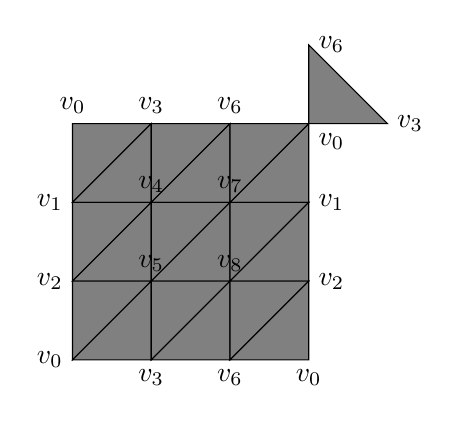
\begin{tikzpicture}
\draw[fill=gray] (0,3) node[anchor=south]{$v_0$} -- (0,2) node[anchor=east]{$v_1$} -- (1,3) -- cycle;
\draw[fill=gray] (0,2) -- (1,3) node[anchor=south]{$v_3$} -- (1,2) -- cycle;
\draw[fill=gray] (1,3) -- (1,2) node[anchor=north]{$v_4$} -- (2,3) node[anchor=south]{$v_6$} -- cycle;
\draw[fill=gray] (1,2) -- (2,3) -- (2,2) -- cycle;
\draw[fill=gray] (2,2) -- (3,3) -- (3,2) node[anchor=west]{$v_1$} -- cycle;
\draw[fill=gray] (3,3) -- (3,4) node[anchor=west]{$v_6$} -- (4,3) node[anchor=west]{$v_3$} -- cycle;
\draw[fill=gray] (2,2) -- (2,3) -- (3,3) node[anchor=north west]{$v_0$} -- cycle;
\draw[fill=gray] (0,2) -- (0,1) node[anchor=east]{$v_2$} -- (1,2) node[anchor=south]{$v_4$} -- cycle;
\draw[fill=gray] (0,1) -- (1,2) -- (1,1) node[anchor=north]{$v_3$} -- cycle;
\draw[fill=gray] (1,2) -- (1,1) node[anchor=north]{$v_5$} -- (2,2) -- cycle;
\draw[fill=gray] (1,1) -- (2,2) node[anchor=south]{$v_7$} -- (2,1) -- cycle;
\draw[fill=gray] (2,1) -- (2,2) -- (3,2) -- cycle;
\draw[fill=gray] (2,1) -- (3,2) -- (3,1) node[anchor=west]{$v_2$} -- cycle;
\draw[fill=gray] (0,1) -- (0,0) node[anchor=east]{$v_0$} -- (1,1) node[anchor=south]{$v_5$} -- cycle;
\draw[fill=gray] (0,0) -- (1,1) -- (1,0) node[anchor=north]{$v_3$} -- cycle;
\draw[fill=gray] (1,1) -- (1,0) -- (2,1) -- cycle;
\draw[fill=gray] (1,0) -- (2,1) -- (2,0) node[anchor=north]{$v_6$} -- cycle;
\draw[fill=gray] (2,0) -- (2,1) node[anchor=south]{$v_8$} -- (3,1) -- cycle;
\draw[fill=gray] (2,0) -- (3,1) -- (3,0) node[anchor=north]{$v_0$} -- cycle;
\end{tikzpicture}
\end{figure}

Hacemos la descomposición obvia con $K_1=T^2$ y $K_2=D^2$, cuya intersección es la circunferencia interior del toro y borde del disco. $H_2(K_1)=\F$ generado por la suma de todos sus 2-símplices y $H_1(K_1)=\F^2$ generado por las dos circunferencias que forman los límites de la triangulación. $H_2(K_2)=H_1(K_1)=0$ por ser colapsable. Por último $H_1(K_1\cap K_2)=\F$. Sustituyendo estos datos en la sucesión de Mayer-Vietoris reducida obtenemos
\[
0\to \F\xrightarrow{j_{*2}}H_2(K)\xrightarrow{\Delta_{2*}}\F\xrightarrow{i_{*1}}\F^2\xrightarrow{j_{*1}}H_1(K)\to 0.
\]
El borde de $K_2$ es evidentemente trivial en $K_2$, pero en $K_1$ es uno de los generadores de la homología, por lo que $i_{*1}$ es inyectiva. Esto implica que $\Delta_{2*}$ es nulo, a lo cual podemos unir el primer teorema de isomorfía para concluir que $H_2(K)=\F$ generado por la suma de los 2-símplices del toro. 

Por otro lado, que $i_{*1}$ sea inyectiva implica que $\ker{j_{*1}}$ tiene rango 1, por lo que por ser además sobreyectiva, esto implica que $H_1(K)=\F$ generado por el 1-ciclo del toro que no es borde de $K_2$. Además $H_0(K)=\F$ por ser conexo. 

\end{solucion}

\newpage

\begin{ejercicio}{2.15}
Triangular el espacio $X ⊆ \R^2$
consistente en $k$ circunferencias disjuntas
$S_1, \dots , S_k$ y un segmento $A$ tangente a cada una de ellas y calcular sus $\F$-espacios
vectoriales de homología.
\end{ejercicio}
\begin{solucion}\

\begin{center}
\begin{tikzpicture}[line cap=round,line join=round,>=triangle 45,x=0.7cm,y=0.7cm]
\clip(.,-1) rectangle (21.,4);
\draw[line width=2.pt] (0.,0.) -- (2.,3.) -- (4.,0.) -- cycle;
\draw[line width=2.pt] (5.,0.) -- (7.,3.) -- (9.,0.) -- cycle;
\draw[line width=2.pt] (14.,0.) -- (16.,3.) -- (18.,0.) -- cycle;
\draw [line width=2.pt] (0.,0.)-- (2.,3.);
\draw [line width=2.pt] (2.,3.)-- (4.,0.);
\draw [line width=2.pt] (4.,0.)-- (0.,0.);
\draw [line width=2.pt] (5.,0.)-- (7.,3.);
\draw [line width=2.pt] (7.,3.)-- (9.,0.);
\draw [line width=2.pt] (9.,0.)-- (5.,0.);
\draw [line width=2.pt] (14.,0.)-- (16.,3.);
\draw [line width=2.pt] (16.,3.)-- (18.,0.);
\draw [line width=2.pt] (18.,0.)-- (14.,0.);
\draw [line width=2.pt] (2.,3.)-- (16.,3.);
\draw (9.74,4.) node[anchor=north west] {$A$};
\draw (1.54,0.) node[anchor=north west] {$S_1$};
\draw (6.7,0.) node[anchor=north west] {$S_2$};
\draw (15.72,0.) node[anchor=north west] {$S_k$};
\begin{scriptsize}
\draw [fill=black] (11.,1.58) circle (1.0pt);
\draw [fill=black] (13.,1.56) circle (1.0pt);
\draw [fill=black] (12.02,1.56) circle (1.0pt);
\end{scriptsize}
\end{tikzpicture}
\end{center}

Este espacio es claramente del mismo tipo de homotopía de un wedge de circunferencias, por lo que su homología es la suma directa de las homologías de las circunferencias, que ya las conocemos.
\end{solucion}

\newpage

\begin{ejercicio}{2.16}
Dados los conjuntos de $\R
^3$
\[
A = \{(x, y, z); x^2 + y^2 + z^2 = 1, x ≤ 0\}\]
\[
B = \{(x, y, z) ∈ \R^3
; x^2 + y^2 + z^2 = 1, x ≥ 0, z = 0\}
\]
sea $X = A
∪
B$. Triangular el espacio $X$ y hallar los $\F$-espacios vectoriales de homología
correspondientes a dicha triangulación.
\end{ejercicio}
\begin{solucion}
Damos la siguiente triangulación $K$

\definecolor{sqsqsq}{rgb}{0.12549019607843137,0.12549019607843137,0.12549019607843137}
\definecolor{eqeqeq}{rgb}{0.8784313725490196,0.8784313725490196,0.8784313725490196}
\begin{tikzpicture}[line cap=round,line join=round,>=triangle 45,x=1.0cm,y=1.0cm]
\clip(-1.87,1) rectangle (9.63,5.61);
\fill[line width=2.pt,color=eqeqeq,fill=eqeqeq,fill opacity=0.800000011920929] (1.28,3.1) -- (2.74,4.5) -- (2.68,1.66) -- cycle;
\fill[line width=2.pt,color=eqeqeq,fill=eqeqeq,fill opacity=0.800000011920929] (2.74,4.5) -- (1.28,3.1) -- (3.52,4.14) -- cycle;
\fill[line width=2.pt,color=eqeqeq,fill=eqeqeq,fill opacity=0.800000011920929] (2.68,1.66) -- (2.74,4.5) -- (4.44,2.96) -- cycle;
\fill[line width=2.pt,color=eqeqeq,fill=eqeqeq,fill opacity=0.800000011920929] (3.52,4.14) -- (2.74,4.5) -- (4.44,2.96) -- cycle;
\draw [line width=2.pt] (1.28,3.1)-- (2.68,1.66);
\draw [line width=2.pt] (2.68,1.66)-- (4.44,2.96);
\draw [line width=2.pt] (2.68,1.66)-- (2.74,4.5);
\draw [line width=2.pt] (1.28,3.1)-- (2.74,4.5);
\draw [line width=2.pt] (2.74,4.5)-- (4.44,2.96);
\draw [line width=2.pt,dash pattern=on 2pt off 2pt] (1.28,3.1)-- (3.52,4.14);
\draw [line width=2.pt] (2.74,4.5)-- (3.52,4.14);
\draw [line width=2.pt] (3.52,4.14)-- (4.44,2.96);
\draw [line width=2.pt,dash pattern=on 2pt off 2pt] (2.68,1.66)-- (3.52,4.14);
\draw [line width=2.pt,color=eqeqeq] (1.28,3.1)-- (2.74,4.5);
\draw [line width=2.pt,color=eqeqeq] (2.74,4.5)-- (2.68,1.66);
\draw [line width=2.pt,color=eqeqeq] (2.68,1.66)-- (1.28,3.1);
\draw [line width=2.pt,color=eqeqeq] (2.74,4.5)-- (1.28,3.1);
\draw [line width=2.pt,color=eqeqeq] (1.28,3.1)-- (3.52,4.14);
\draw [line width=2.pt,color=eqeqeq] (3.52,4.14)-- (2.74,4.5);
\draw [line width=2.pt,color=eqeqeq] (2.68,1.66)-- (2.74,4.5);
\draw [line width=2.pt,color=eqeqeq] (2.74,4.5)-- (4.44,2.96);
\draw [line width=2.pt,color=eqeqeq] (4.44,2.96)-- (2.68,1.66);
\draw [line width=2.pt,color=eqeqeq] (3.52,4.14)-- (2.74,4.5);
\draw [line width=2.pt,color=eqeqeq] (2.74,4.5)-- (4.44,2.96);
\draw [line width=2.pt,color=eqeqeq] (4.44,2.96)-- (3.52,4.14);
\draw [line width=2.pt] (1.28,3.1)-- (2.74,4.5);
\draw [line width=2.pt] (2.74,4.5)-- (2.68,1.66);
\draw [line width=2.pt] (2.68,1.66)-- (1.28,3.1);
\draw [line width=2.pt] (2.74,4.5)-- (4.44,2.96);
\draw [line width=2.pt] (4.44,2.96)-- (2.68,1.66);
\draw [line width=2.pt] (2.74,4.5)-- (3.52,4.14);
\draw [line width=2.pt,color=sqsqsq] (3.52,4.14)-- (4.44,2.96);
\end{tikzpicture}

donde el poliedro es hueco y el ``suelo'' no tiene 2-símplices.

Descomponemos $K$ como las triangulaciones correspondientes a $A$ y a $B$, es decir, el cono sobre el cuadrilátero y el segmento transveral. Ambas homologías reducidas son triviales, y la intersección son dos puntos, que tiene homología reducida trivial en todos los niveles salvo en el 0, que es $\F$.  Así que obtenemos que 
\[
\widetilde{H}_n(K,\F)\cong \begin{cases}
\F & n=1\\
0 & c.c.
\end{cases}
\]
donde $\F$ está generado por la circunferencia sobre la que colapsa el complejo, que es la circunferencia formada por el segmento transveral y las dos aristas con las que es incidente. 
\end{solucion}
\newpage

\begin{ejercicio}{2.17}
Dado el espacio $Y = A
∪
B$, donde
\[
A = \{(x, y, z) ∈ \R^3
; x^2 + y^2 + z^2 = 1\}
\]
\[
B = \{(x, y, z) ∈ \R^3
; x = 0, z = 0, −1 ≤ y ≤ 1\}
\]
triangular $Y$ y hallar los $\F$-espacios vectoriales de homología correspondientes a esa triangulación
\end{ejercicio}
\begin{solucion}
Este espacio se puede triangular uniendo dos tetraedos por sus ``suelos'' y conectando los dos vértices no adyacentes con una arista. 

\begin{figure}[h]
\centering
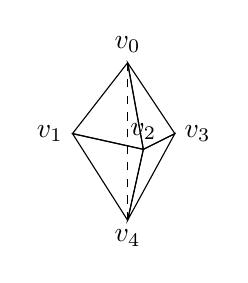
\begin{tikzpicture}
\draw (1,2) node[anchor=south]{$v_0$} -- (0.3,1.1) node[anchor=east]{$v_1$} -- (1.2,0.9) -- cycle;
\draw (1.2,0.9) node[anchor=south]{$v_2$} -- (1.6,1.1) node[anchor=west]{$v_3$}-- (1,2) -- cycle; 
\draw (1.2,0.9) -- (1.6,1.1) -- (1,0) node[anchor=north]{$v_4$} -- cycle; 
\draw (1,0) -- (0.3,1.1) -- (1.2,0.9) -- cycle; 
\draw[dashed] (1,0) -- (1,2); 
\end{tikzpicture}
\end{figure}

Tomamos $K_1 = (v_0, v_4)$ y $K_2 \cong$ triangulación de las esfera.
Entonces $K = K_1 \cup K_2$ y $K_1 \cap K_2 = \{(v_0), (v_4)\}$.

Usando Mayer-Vietoris reducido teniendo en cuenta que:
\begin{itemize}
\item $\widetilde{H}_2(K_1 \cap K_2) = 0$.
\item $\widetilde{H}_2(K_1) \oplus \widetilde{H}_2(K_2) = 0 \oplus \F\gene{c} \cong \F\gene{c}$.
\item $\widetilde{H}_1(K_1 \cap K_2) = 0$.
\item $\widetilde{H}_1(K_1) \oplus \widetilde{H}_2(K_2) = 0$.
\item $\widetilde{H}_0(K_1 \cap K_2) = \F\gene{v_0-v_4}$.
\item $\widetilde{H}_0(K_1) \oplus \widetilde{H}_0(K_2) = 0$.
\end{itemize}
Donde $c$ suma es la súma de los símplices de $K$ de dimensión $2$
Tenemos que:
\[ 0 \xrightarrow{i_{*2}} \F\gene{c} \xrightarrow{j_{*2}} \widetilde{H}_2(K) \xrightarrow{\Delta_2} 0 \]
\[ 0 \xrightarrow{j_{*1}} \widetilde{H}_1(K) \xrightarrow{\Delta_1} \F\gene{v_0-v_4} \xrightarrow{i_{*0}} 0 \]
\[ 0 \xrightarrow{j_{*0}} \widetilde{H}_0(K) \to 0 \]
Por lo tanto, $\widetilde{H}_2(K) = \F\gene{c}$, $\widetilde{H}_1(K) = \F\gene{v_0-v_4}$ y $\widetilde{H}_0(K) = 0$.
\end{solucion}

\newpage

\begin{ejercicio}{2.18}
Sea $X$ el subespacio de $\R^3$
consistente en una esfera encajada por
su ecuador en un toro. Triangular $X$ y calcular los $\F$-espacios vectoriales de homología
simplicial de $X$. Determinar también la carcaterística de Euler-Poincaré $χ(K)$.
\end{ejercicio}
\begin{solucion}
A partir de la triangulación del ejercicio \ref{ejer:2.14} basta tomar un vértice $v_9$ afinmente independiente a $\{v_0,v_3,v_6\}$ y hacer con esto la triangulación habitual de la esfera sobre el disco triangulado que se añadió a la triangulación del toro. Entonces hacemos la descomposición análoga a dicho ejercicio. Ahora $H_2(K_2)=\F$ y $H_1(K_1)=0$. La intersección sigue siendo la misma que en el anteriomente mencionado ejercicio. Lo que nos da la sucesión de Mayer-Vietoris reducida
\[
0\to \F\oplus\F\xrightarrow{j_{*2}}H_2(K)\xrightarrow{\Delta_{2*}}\F\xrightarrow{i_{*1}}\F^2\xrightarrow{j_{*1}}H_1(K)\to 0.
\]
De nuevo $i_{*1}$ actúa como en el \ref{ejer:2.14} por lo que los cálculos son análogos, obteniendo así $H_2(K)=\F^2$ generado por el generador de la del toro y la de la esfera, y $H_1(K)=\F$ generado por el ciclo del toro que no interseca en la esfera. Como de costumbre, $H_0(K)=\F$.

Con todo esto, $\chi(K)=1-1+2=2$.  
\end{solucion}

\newpage

\begin{ejercicio}{2.19}
Calcular los $\F$-espacios vectoriales de homología de un cilindro con dos
agujeros.
\end{ejercicio}
\begin{solucion}
Un cilindro al que se le hacen dos agujeros es del mismo tipo de homotopía que de un wedge de tres circunferencias, por lo que sus espacios de homología son las sumas directas de los de las tres circunferencias. 
\end{solucion}

\newpage

\begin{ejercicio}{2.20}
Calcular los $\F$-espacios vectoriales de homología de:

\begin{figure}[h!]
\centering
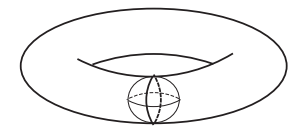
\includegraphics[scale=0.7]{toro1}
\end{figure}
\end{ejercicio}
\begin{solucion}
El cálculo es análogo al ejercicio \ref{ejer:2.18} ya que la triangulación es similar, pero intercambiando $v_3$ por $v_1$ y $v_6$ por $v_2$, así que resulta la misma homología. 

\end{solucion}

\newpage

\begin{ejercicio}{2.21}
Calcular los $\F$-espacios vectoriales de homología de dos toros entrelazados:

\begin{figure}[h!]
\centering
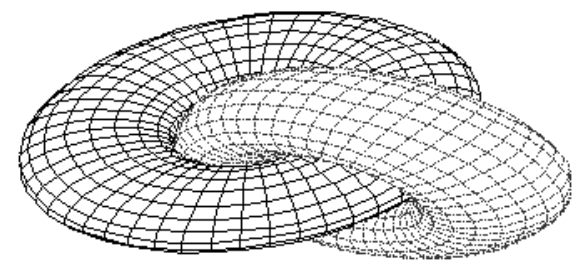
\includegraphics[scale=0.5]{toro2}
\end{figure}
\end{ejercicio}

\begin{solucion}
Para triangular este espacio basta considerar dos toros disjuntos triangulados e identificar de la misma forma los lados superior e inferior de uno con los laterales del otro. Esto nos da una descomposición evidente del espacio de la figura como unión de dos toros cuya intersección es una cirfunferencia. Mayer-Vietoris nos da la sucesión exacta

\begin{align*}
0\to\F\oplus\F\xrightarrow{j_{*2}} H_2(K)\xrightarrow{\Delta_{*2}}\F\xrightarrow{i_{*1}}(\F\oplus\F)\oplus(\F\oplus\F)\xrightarrow{j_{*1}}H_1(K)\to 0
\end{align*}

Como la circunferencia de la intersección no es borde en la unión, $i_{*1}$ es inyectiva, por lo que $\ker{i_{i*}}=\Ima\Delta_{*2}=0$. Esto significa que $rango H_2(K)=rango(\ker\Delta_{*2})=rango(\Ima{j_{2*}})=2$, de modo que $H_2(K)\cong \F\oplus\F$ generada por cada uno de los dos toros. Por exactitud hemos obtenido a su vez que $\ker{j_{1*}}=\F$, luego $H_1(K)=\F\oplus\F\oplus\F$, generada por cada una de las tres circunferencias que aparecen identificadas. Claramente $H_0(K)=\F$. 
\end{solucion}

\newpage

\begin{ejercicio}{2.22}
Probar que los espacios euclídeos $\R^n$
y $\R^m$ no son homeomorfos si $n\neq m$.
\end{ejercicio}
\begin{solucion}
Si fueran homeomorfos también serían homeomorfos $\R^n-\{x\}$ y $\R^m-\{y\}$ donde $x\in\R^n$ e $y\in\R^m$. Sabemos que estos espacios son del mismo tipo de homotopía que $S^{n-1}$ y $S^{m-1}$ respectivamente, por lo que conocemos sus espacios de homología, los cuales sabemos que no son iguales si $n\neq m$, por lo que no $\R^n$ no es homeomorfo a $\R^m$ en este caso.
\end{solucion}
\newpage

\begin{ejercicio}{2.23}
Dar un ejemplo de dos espacios topológicos no homeomorfos pero que
tengan todos sus $\F$-espacios vectoriales de homología isomorfos.
\end{ejercicio}
\begin{solucion}
Considerar las realizaciones geométricas de los complejos del ejercicio \ref{ejer:2.4}.
\end{solucion}


\end{document}
